% Keeping the Red Red — research paper sources.
% Compiles with pdflatex + bibtex (acmart, sigconf, nonacm): Overleaf, arXiv, TeX Live 2023+.
% See README.md in this folder.
\documentclass[sigconf,nonacm,screen]{acmart}

\usepackage{booktabs}
\usepackage{tabularx}
\usepackage{amsmath}
\usepackage{pgfplots}
\pgfplotsset{compat=1.18}

\settopmatter{printacmref=false}
% Running head: a preprint, not a conference (replaces acmart's "Conference'17" placeholder).
\acmConference[Preprint]{}{October 2026}{}
\acmYear{2026}

\begin{document}

\title[Keeping the Red Red]{Keeping the Red Red: Colour Loss, Perceptual Quality Targets and Deployment Constraints in a Self-Hosted Storefront Image Pipeline}

\author{Ahmed Trad}
\affiliation{%
  \institution{Independent researcher}
  \country{Spain}}
\email{tradahmed1995@gmail.com}

\begin{abstract}
Self-hosted storefronts compress and resize every product photo they serve, and the tools that do it treat quality as a preset and ignore the colour profile inside the file. We study one WooCommerce store on shared hosting end to end: an image pipeline built on the three core WordPress filters that also govern the browser-side processing introduced in WordPress 7.1, a measurement method for the colour loss that occurs when a wide-gamut profile is dropped, and a calibration of encoder quality against structural similarity per product category. The pipeline cut a 93-image library from 126.6\,MB to 87.3\,MB in WebP with no visible loss. In that library 13 photos (14\%) carry a Display P3 profile, far above the 0.4\% share reported for the web; on a GD host, which drops profiles, two of them shift every pixel by a mean $\Delta E_{76}$ of 6 to 7, well past the just-noticeable distance. A crawl of 68 live modest-fashion stores (26 with a public catalogue, 2,419 images) found wide-gamut profiles on only 0.5\% of served images and no loss in the wild: Shopify converts its resized copies to sRGB and the one self-hosted store with such uploads keeps the profile on resize. The common defect there is size, with 19\% of full-size product images narrower than 900\,px. The calibration shows that the spread of structural similarity inside a category is as wide as the gap between categories, so a per-image perceptual target is the only setting that is both small and safe. Testing both upload paths of WordPress 7.1 exposed a sequencing defect that orphans the untouched upload when an image is both converted and scaled, and we give the correction. Finally we analyse the constraints a browser-side pipeline inherits: cross-origin isolation, which limits it to Chromium today; the cost of a perceptual metric in WebAssembly; and the absence of a reliable colour transform on shared hosting. The code is public.
\end{abstract}

\keywords{image optimisation, colour management, Display P3, ICC profiles, perceptual quality, WebP, WordPress, WooCommerce, WebAssembly, cross-origin isolation}

\maketitle

\section{Introduction}

Images are the largest thing a storefront sends to a phone and the thing a shopper judges a product by. On the median mobile page the largest contentful paint is an image 68\% of the time, and the heaviest image per page has grown 13\% in two years~\cite{almanac2024media}. A fashion store adds a concern that performance work ignores: the colour on the screen has to be the colour in the parcel, or the parcel comes back.

Two developments make this a timely problem for self-hosted shops. First, WordPress 7.1 moved image resizing, conversion and thumbnail generation into the browser, using libvips compiled to WebAssembly, for Chromium browsers that support document isolation~\cite{wp71devnote}. Second, the commercial image optimisers for WordPress sell the same encoder layer that the platform now provides, expose quality as three presets, and do not manage colour profiles at all~\cite{shortpixelkb}.

This paper reports a complete investigation on one store, a modest-fashion boutique selling in three languages from shared hosting; the merchant is not named. We built the pipeline into its theme, measured it, and analysed what a product built on the same foundations would run into. Our contributions are:

\begin{enumerate}
  \item A pipeline on the three core filters that govern both the server-side and the browser-side processing paths (Section~\ref{sec:pipeline}), with reversible library conversion, and the identification and correction of a sequencing defect in the WordPress 7.1 finalize step (Section~\ref{sec:paths}).
  \item A measurement method for the colour loss caused by dropping a wide-gamut profile: parsing the embedded ICC profile from the file itself and computing $\Delta E_{76}$ between the image read through its profile and read as sRGB (Section~\ref{sec:colourmethod}), validated with real and synthetic profiles (Section~\ref{sec:colourresults}).
  \item Pilot measurements in a real product library: prevalence of Display P3 photos and the size of their shift (Section~\ref{sec:colourresults}).
  \item A per-category calibration of WebP quality against structural similarity that argues for per-image perceptual targets (Section~\ref{sec:calibration}).
  \item An analysis of the deployment constraints of a browser-side pipeline: cross-origin isolation and browser support, the cost of a perceptual metric in WebAssembly, and the routes to a colour transform on shared hosting (Section~\ref{sec:constraints}).
\end{enumerate}

\section{Background and related work}

\subsection{Formats and delivery}

At equal visual quality measured by DSSIM, WebP files are a median 31\% smaller than JPEG and AVIF 50\% smaller, over 600 photographs at six sizes; AVIF encodes five to twenty times slower~\cite{aleksandersen2020}. Google's A/B test of WordPress's default lazy loading found that lazy-loading images above the fold delays the largest contentful paint, and that excluding them cut an archive template's LCP from 1,657 to 1,352\,ms~\cite{webdevlazy}; 9.5\% of mobile LCP images are still lazy-loaded~\cite{almanac2024media}. Responsive image candidates let a 375\,px phone fetch 80\,KB instead of 254\,KB for one photograph~\cite{nearform2019}, while inaccurate \texttt{sizes} attributes waste a median 16\% on mobile and mis-select candidates on one page in five~\cite{almanac2024media}. Image CDNs claim 40 to 80\% savings, mostly from per-device resizing and format negotiation~\cite{webdevcdn}, which a pipeline that resizes and converts itself already provides.

\subsection{Perceptual quality metrics}

SSIM compares local means, variances and covariances of luminance and correlates with perceived quality better than PSNR~\cite{wang2004ssim}. SSIMULACRA~2 is a multi-scale metric in the XYB opponent colour space designed for compression artefacts; its predecessor agreed with human judgement in 87\% of pairwise cases against 82\% for DSSIM and 80\% for Butteraugli~\cite{sneyers2017psychovisual,sneyers2023ssimulacra2}, and its scale reads 100 for identical images, 90 and above for imperceptible differences, and below 50 for clearly degraded ones~\cite{fastssim2}. Single-threaded reference implementations take about 350 to 380\,ms per 1080p comparison on a current desktop processor~\cite{zensim}. A verification pipeline that re-encodes until the score passes has been described for a server-side optimiser~\cite{modpagespeed}.

\subsection{Colour management on the web}

An ICC profile describes a device colour space by, for matrix/TRC profiles, three primaries adapted to the D50 connection space and three tone reproduction curves~\cite{icc2010}. Browsers interpret untagged image data as sRGB; the 2024 Web Almanac reports 87.7\% of mobile images without a profile, Display P3 at 0.4\% and Adobe RGB at 0.7\%~\cite{almanac2024media}. Display P3 is the capture and display space of Apple devices since 2016~\cite{iccdisplayp3}. The CIE 1976 colour difference $\Delta E_{76}$ is the Euclidean distance in CIELAB; a difference of about 2.3 is the usual just-noticeable threshold~\cite{mokrzycki2011}, and CIEDE2000 refines it for small differences~\cite{sharma2005ciede}. The PHP GD library has no colour management and drops profiles; ImageMagick converts between profiles only when built with the LittleCMS delegate, and silently does nothing otherwise~\cite{phpimagick}. WordPress's Imagick editor strips metadata from the sizes it writes but keeps the ICC, IPTC, EXIF and XMP profiles since version 4.5, so a wide-gamut upload resized by Imagick keeps its profile and a browser still honours it~\cite{wptrac33642,wptrac58435}; GD has no such path. Hosted platforms handle this on their own: Shopify's help page says the colour profile of an uploaded image is removed and sRGB assumed~\cite{shopifycolors}; what its CDN actually serves is measured in Section~\ref{sec:crawl}. Before an image reaches any store it has often passed through a messaging application, and the forensics literature documents that those recompress images and remove their metadata, to the point that the processing chain can be identified from the file~\cite{giudice2017ballistics,pasquini2021survey}; such a file arrives untagged whatever its camera's colour space was.

\subsection{Client-side processing and isolation}

WordPress 7.1 processes uploads in the browser with wasm-vips, a WebAssembly build of libvips that requires \texttt{SharedArrayBuffer} for its threads~\cite{wasmvips,libvipswasm}. Browsers have gated \texttt{SharedArrayBuffer} behind cross-origin isolation since Spectre, because a shared buffer is a high-resolution timer and a timer makes cache side channels practical~\cite{kocher2019spectre,webdevcoop}. Isolation is declared with the \texttt{Cross-Origin-Opener-Policy} and \texttt{Cross-Origin-Embedder-Policy} headers, which cut the page off from cross-origin popups and require every embedded resource to opt in. Document-Isolation-Policy isolates one document without demands on its subframes; it shipped in Chrome 137 and is incubated in the WICG~\cite{chromedip,tag995}.

\section{Method}

\subsection{Setting}

The subject is the store's bespoke WooCommerce theme and a local copy of the store: WordPress 7.1.3, PHP 8.2.12, the bundled GD 2.1 with WebP and AVIF support, no ImageMagick, Apache on Windows. The library holds 93 product images (86 JPEG, 7 PNG), mostly $896\times1195$ product photographs across seven categories (chiffon hijabs, premium jersey, printed modal, abayas, jewellery and accessories). Browser tests ran in Playwright~1.50 with Edge~155 (Chromium) and WebKit~18.

\subsection{Pipeline}
\label{sec:pipeline}

Nothing in the theme converts an image itself. WordPress's image editor does, through three core filters answered from one option: \texttt{image\_editor\_output\_format} maps JPEG and PNG to WebP (or AVIF when the server can write it), \texttt{big\_image\_size\_threshold} sets the longest side (2048\,px), and \texttt{wp\_editor\_set\_quality} sets the encoder quality (82; AVIF receives 80\% of it). WordPress 7.1 exposes the same three answers to the browser through its REST attachment schema, so the server path and the browser path produce the same files.

The upload is always kept next to what the site serves, as core keeps the original of a scaled image. Images uploaded before the change are rebuilt from their kept originals with core's own regeneration routine in resumable five-second batches; the files an image served before stay on disk, listed per attachment, until a separate removal step, so cached pages and old links keep working. Choosing the uploaded format and converting again restores the previous state. Two storefront details follow from a format change: the Open Graph share image is kept as a JPEG copy because WhatsApp shows no preview for WebP or AVIF, and image tags stored in content with the file name they had at insertion are pointed at the current file of the same size.

\subsection{Profile extraction and parsing}
\label{sec:profilemethod}

The profile is read from the file itself, without an imaging library, so that the measurement does not depend on what the host's editor preserves. JPEG profiles are the concatenation of the numbered \texttt{APP2} segments tagged \texttt{ICC\_PROFILE}; PNG profiles are the zlib stream of the \texttt{iCCP} chunk; WebP profiles are the \texttt{ICCP} chunk of the RIFF container. The parser reads the header, the tag table, the \texttt{rXYZ}, \texttt{gXYZ} and \texttt{bXYZ} columns as s15Fixed16 numbers, the three TRC tags (\texttt{curv} with a gamma, a table, or \texttt{para} with parametric types 0 to 4), and the description (\texttt{desc} in version 2, \texttt{mluc} in version 4).

A profile is classed as sRGB when every element of its matrix is within 0.02 of the sRGB matrix adapted to D50,
\begin{equation}
M_{\mathrm{sRGB}} =
\begin{pmatrix}
0.4360747 & 0.3850649 & 0.1430804\\
0.2225045 & 0.7168786 & 0.0606169\\
0.0139322 & 0.0971045 & 0.7141733
\end{pmatrix}.
\end{equation}
The description is consulted only when a profile has no matrix. This rule matters in practice: the profile named ``Display P3 Gamut with sRGB Transfer'', common in phone exports, contains the letters sRGB and is P3.

\subsection{Colour-loss measure}
\label{sec:colourmethod}

For a pixel with encoded channel values $v_c \in [0,1]$, the colour the file intends is obtained by linearising each channel through the profile's tone curve $T_c$ and applying the profile's matrix $M_p$,
\begin{equation}
\mathbf{X}_p = M_p\,\big(T_R(v_R),\,T_G(v_G),\,T_B(v_B)\big)^{\mathsf T},
\end{equation}
while the colour a browser shows once the profile is gone is
\begin{equation}
\mathbf{X}_s = M_{\mathrm{sRGB}}\,\big(E(v_R),\,E(v_G),\,E(v_B)\big)^{\mathsf T},
\end{equation}
with $E$ the sRGB electro-optical transfer function. Both are converted to CIELAB with the D50 white point $(0.9642, 1.0000, 0.8249)$ and the loss is
\begin{equation}
\Delta E_{76} = \lVert \mathrm{Lab}(\mathbf{X}_p) - \mathrm{Lab}(\mathbf{X}_s) \rVert_2 .
\end{equation}
The image is sampled by area-resampling its smallest generated size, which carries the same pixel values as the original, to at most $48\times48$ pixels, and three statistics are reported: the mean, the 95th percentile, and the share of pixels with $\Delta E_{76} > 2.3$. The same sample yields the image's average colour, which the storefront paints behind the image while it loads.

\subsection{Calibration protocol}
\label{sec:calibmethod}

For each product category, up to six featured photographs were cropped to the $600\times800$ card size the storefront serves, written losslessly as the reference, and encoded as WebP at qualities 60, 68, 76, 82, 88 and 94. Each encoding was compared with the reference by SSIM on luminance ($Y = 0.299R + 0.587G + 0.114B$) at half size, with $8\times8$ windows at stride 4 and the standard constants $C_1=(0.01\cdot255)^2$, $C_2=(0.03\cdot255)^2$. The variance of the Laplacian of the reference's luminance was recorded as a measure of fine detail.

\subsection{Upload-path protocol}

Two images, an $896\times1195$ product photograph and a $3000\times2000$ synthetic JPEG, were uploaded through the block editor in Edge (document isolation active, browser-side processing) and in WebKit (no isolation, server-side fallback), with every media REST request recorded and the resulting attachment metadata and files inspected after the editor's finalize call.

\section{Results}

\subsection{Pipeline outcomes}

Converting the 93-image library to WebP through the screen took 559\,s, about 6\,s per $896\times1195$ photograph with fourteen sizes each, and reduced it from 126.6\,MB to 87.3\,MB (31\%); converting back took 267\,s; removing the 1,289 superseded files freed 87.3\,MB. In the command-line interpreter the same photograph rebuilds in 2.8\,s, so about half of the cost on the web path is the web server's PHP rather than the encoder.

\subsection{Upload paths and a sequencing defect}
\label{sec:paths}

Table~\ref{tab:paths} summarises the two paths. The browser path converts and scales as configured, with each size sideloaded by the browser and a finalize call at the end. For an image that is both converted and scaled, however, the server converts the first upload and records the untouched JPEG as the original, and the later ``scaled'' sideload overwrites that record with the converted full-size file; the JPEG is left on disk unreferenced and is not deleted with the attachment. The correction runs on the metadata filter that finalize applies last: when the recorded original has an extension that does not match the attachment's uploaded type and a sibling file with the uploaded type's extension exists, the sibling is restored as the original and the superseded converted file is deleted. After the correction the browser path produced the same files as the server path.

\begin{table}[t]
\caption{Both upload paths after the correction (WordPress 7.1.3), $3000\times2000$ JPEG upload.}
\label{tab:paths}
\small
\begin{tabularx}{\columnwidth}{@{}lXX@{}}
\toprule
Browser & Path taken & Outcome \\
\midrule
Edge 155 & Browser: 17 sideloads, then finalize & Scaled WebP at 2048\,px, 16 sizes, JPEG kept \\
WebKit 18 & Server: silent fallback, 66\,s & Scaled WebP at 2048\,px, 17 sizes, JPEG kept \\
\bottomrule
\end{tabularx}
\end{table}

\subsection{Quality calibration by category}
\label{sec:calibration}

\begin{table}[t]
\caption{Mean file size (KB) and SSIM of the $600\times800$ WebP card crop by category and quality; $n$ photographs per category; detail is the Laplacian variance of the reference.}
\label{tab:calib}
\footnotesize
\setlength{\tabcolsep}{3.5pt}
\begin{tabular}{@{}llrrrrrr@{}}
\toprule
Category ($n$, detail) & & q60 & q68 & q76 & q82 & q88 & q94 \\
\midrule
Chiffon hijabs (6, 551) & KB & 37.8 & 42.0 & 48.6 & 61.9 & 80.5 & 116.1 \\
 & SSIM & 0.9653 & 0.9706 & 0.9765 & 0.9854 & 0.9913 & 0.9956 \\
Premium jersey (6, 140) & KB & 9.1 & 10.1 & 11.7 & 15.4 & 22.9 & 42.7 \\
 & SSIM & 0.9823 & 0.9837 & 0.9855 & 0.9881 & 0.9912 & 0.9946 \\
Printed modal (6, 504) & KB & 19.9 & 22.2 & 25.4 & 33.2 & 45.3 & 74.2 \\
 & SSIM & 0.9823 & 0.9849 & 0.9874 & 0.9910 & 0.9940 & 0.9966 \\
Bracelets (1, 729) & KB & 11.2 & 12.8 & 14.5 & 18.3 & 23.8 & 33.9 \\
 & SSIM & 0.9727 & 0.9791 & 0.9830 & 0.9904 & 0.9947 & 0.9975 \\
Necklaces (2, 710) & KB & 33.5 & 38.3 & 47.0 & 65.4 & 95.0 & 143.0 \\
 & SSIM & 0.9339 & 0.9431 & 0.9547 & 0.9708 & 0.9872 & 0.9947 \\
\bottomrule
\end{tabular}
\end{table}

\begin{figure}[t]
\centering
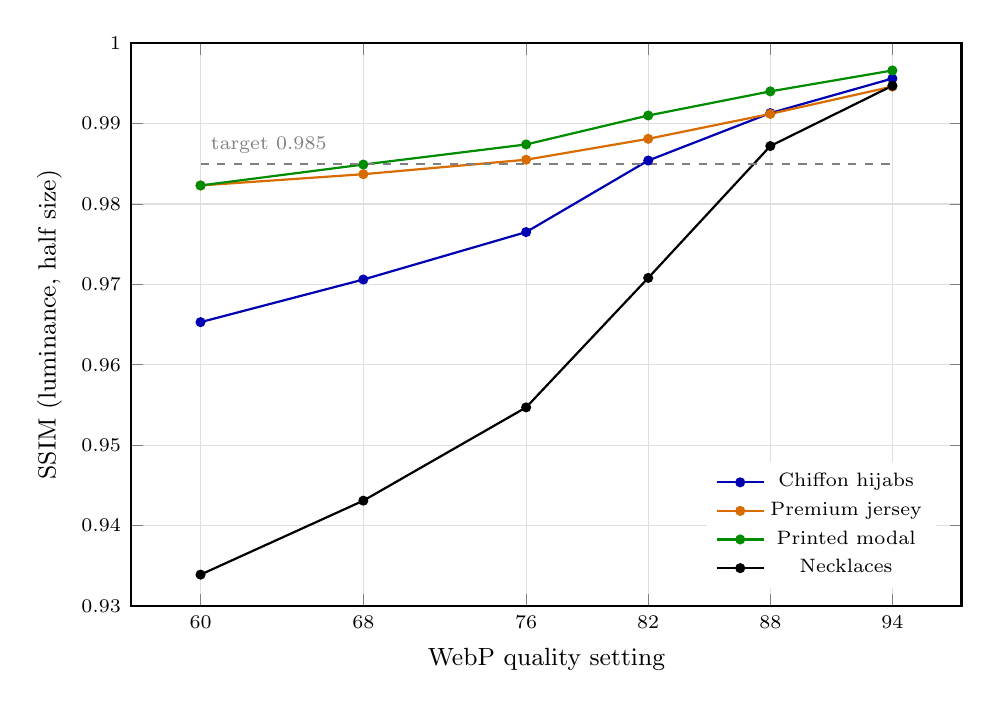
\begin{tikzpicture}
\begin{axis}[
  width=\columnwidth, height=0.72\columnwidth,
  xlabel={WebP quality setting}, ylabel={SSIM (luminance, half size)},
  xtick={60,68,76,82,88,94}, ymin=0.93, ymax=1.0,
  grid=major, grid style={gray!25},
  legend pos=south east, legend style={font=\scriptsize, draw=none},
  tick label style={font=\scriptsize}, label style={font=\small},
  mark size=1.4pt, line width=0.8pt]
\addplot[color=blue!70!black, mark=*] coordinates {(60,0.9653) (68,0.9706) (76,0.9765) (82,0.9854) (88,0.9913) (94,0.9956)};
\addlegendentry{Chiffon hijabs}
\addplot[color=orange!85!black, mark=*] coordinates {(60,0.9823) (68,0.9837) (76,0.9855) (82,0.9881) (88,0.9912) (94,0.9946)};
\addlegendentry{Premium jersey}
\addplot[color=green!55!black, mark=*] coordinates {(60,0.9823) (68,0.9849) (76,0.9874) (82,0.9910) (88,0.9940) (94,0.9966)};
\addlegendentry{Printed modal}
\addplot[color=black, mark=*] coordinates {(60,0.9339) (68,0.9431) (76,0.9547) (82,0.9708) (88,0.9872) (94,0.9947)};
\addlegendentry{Necklaces}
\addplot[dashed, gray, no markers, forget plot] coordinates {(60,0.985) (94,0.985)};
\node[font=\scriptsize, gray, anchor=south west] at (axis cs:60,0.985) {target 0.985};
\end{axis}
\end{tikzpicture}
\caption{SSIM against WebP quality per category. Jersey and modal reach 0.985 at q76, chiffon at q82, necklaces at q88 (Table~\ref{tab:calib}).}
\label{fig:calib}
\end{figure}

Table~\ref{tab:calib} and Figure~\ref{fig:calib} give the results. Categories differ as expected from their detail: at one target of SSIM $\geq 0.985$, chiffon stays at q82, jersey and printed modal reach it at q76 with 24\% and 23\% fewer bytes, and necklaces need q88 at 45\% more bytes; jewellery on a busy background is the most demanding content in the store and is served below the rest at today's single setting. The spread inside a category is as wide as the gap between categories: within chiffon alone, SSIM at q82 runs from 0.982 to 0.992 and detail from 50 to 1194. Per-category presets would therefore both waste bytes and under-serve individual photographs; a per-image target does neither.

\subsection{Colour loss}
\label{sec:colourresults}

\textbf{Validation.} The method was checked both ways with Windows' own sRGB, Adobe RGB (1998) and ProPhoto RGB profiles, and a synthesised Display P3 profile with parametric sRGB-type curves, each spliced into the same dark-red product photograph as JPEG \texttt{APP2} segments and as a PNG \texttt{iCCP} chunk (Table~\ref{tab:validation}). An sRGB profile read as itself yields $\Delta E_{76}=0$; pure P3 primaries shift by more than 10 while greys do not move; the three wide-gamut profiles order as their gamuts do.

\begin{table}[t]
\caption{Colour loss measured on one dark-red product photograph with each profile embedded; share = pixels with $\Delta E_{76} > 2.3$.}
\label{tab:validation}
\small
\begin{tabular}{@{}lrrr@{}}
\toprule
Profile & Mean $\Delta E_{76}$ & 95th pct. & Share \\
\midrule
sRGB IEC61966-2.1 & 0.0 & 0.0 & 0\% \\
Display P3 (synthesised) & 3.1 & 6.5 & 38\% \\
Adobe RGB (1998) & 5.1 & 10.5 & 95\% \\
ProPhoto RGB & 17.7 & 35.6 & 100\% \\
\bottomrule
\end{tabular}
\end{table}

\textbf{Prevalence.} Of the 93 library images, 80 carry no profile and 13 (14\%) carry a Display P3 profile: three named ``Display P3'' and ten named ``Display P3 Gamut with sRGB Transfer''. The first version of the detector trusted the name and missed the ten; the primaries now decide. Table~\ref{tab:library} lists the worst five. Two photographs shift every pixel past the noticeable threshold with a mean of 6 to 7; on a GD host every size made from them is served with that shift.

\begin{table}[t]
\caption{The five photographs with the largest measured shift in the library (all Display P3).}
\label{tab:library}
\small
\begin{tabular}{@{}lrrr@{}}
\toprule
Photograph & Mean $\Delta E_{76}$ & 95th pct. & Share \\
\midrule
P1 (hijab, pink) & 6.8 & 7.5 & 100\% \\
P2 (hijab, red) & 5.9 & 7.7 & 100\% \\
P3 (hijab, rose) & 4.7 & 5.2 & 100\% \\
P4 (dress, burgundy) & 2.5 & 5.9 & 45\% \\
P5 (hijab, mauve) & 2.5 & 2.7 & 94\% \\
\bottomrule
\end{tabular}
\end{table}

\subsection{Live stores}
\label{sec:crawl}

Across live stores the colour problem is rare and the size problem is common. From a list of 217 addresses of European modest-fashion stores, 68 resolved; 26 published a catalogue the crawler could read (23 through Shopify's public \texttt{/products.json}, 3 through the WooCommerce Store API), 39 published none and 3 forbid it in \texttt{robots.txt}. On 15 October 2026 the crawler measured 2,419 full-size product images, at most 100 per store, from the first 128\,KB of each file (Table~\ref{tab:crawl}), reading only public catalogues and honouring the Robots Exclusion Protocol~\cite{rfc9309}; a documented sampling frame for a larger study is the HTTP Archive's monthly crawl with its detected technologies and site rank~\cite{httparchive}.

\begin{table}[t]
\caption{Live stores by how their files are served: profile tags on the full-size image, median served width, and the share narrower than 900\,px.}
\label{tab:crawl}
\footnotesize
\setlength{\tabcolsep}{4pt}
\begin{tabular}{@{}lrrrrrrr@{}}
\toprule
Served by & Stores & Images & sRGB & None & Wide gamut & Median px & $<$900\,px \\
\midrule
Shopify CDN & 23 & 2,211 & 91.9\% & 7.7\% & 10 (0.5\%) & 1,536 & 15.6\% \\
Self-hosted & 3 & 208 & 13.5\% & 85.1\% & 3 (1.4\%) & 752 & 51.0\% \\
\bottomrule
\end{tabular}
\end{table}

Wide-gamut profiles appeared on 13 images in two stores, all Display P3. For each, the crawler also fetched the store's resized copy and parsed its profile. Shopify serves the original with its profile and tags every resized copy sRGB (10 of 10, a compact sRGB profile). A tag alone would be a loss, so for the two images with the largest shift we fetched the full original and the CDN's 300\,px copy, downscaled the original ourselves without colour management and compared the two pixel by pixel in CIELAB: the CDN copy sits $\Delta E$ 1.2 and 1.3 from the original read through its profile, and 3.0 and 5.5 from the original read as sRGB, so the pixels were converted, not merely re-tagged. Shopify's help page says the profile is removed~\cite{shopifycolors}; what is served is a conversion. The WooCommerce store keeps the profile in its resized copies (3 of 3), as ImageMagick does, so browsers honour it. No loss was observed in the wild. The loss measured in Section~\ref{sec:colourresults} needs two things together, an editor that drops profiles and uploads that come straight from a phone, and this sample contained neither: 85\% of self-hosted uploads carry no profile at all, which is what photographs look like after a messaging app or export tool has stripped them, and which hides any shift that happened before upload.

Size is the common defect (Figure~\ref{fig:widths}). 18.6\% of full-size product images are narrower than 900\,px and 38.3\% narrower than 1,200\,px; three stores serve most of their catalogue below 900\,px (one Shopify store 95 of 99 images, another 64 of 100, the self-hosted balkiss.com all 100 at 752\,px). WooCommerce's default single-product image is 600\,px wide and themes commonly ask for more~\cite{woosizes}; on any theme whose product box is wider than the served file, those photographs are enlarged by the browser. The share is a store property more than an image property: the median store serves 3\% of its images below 900\,px and three stores serve more than half.

\begin{figure}[t]
\centering
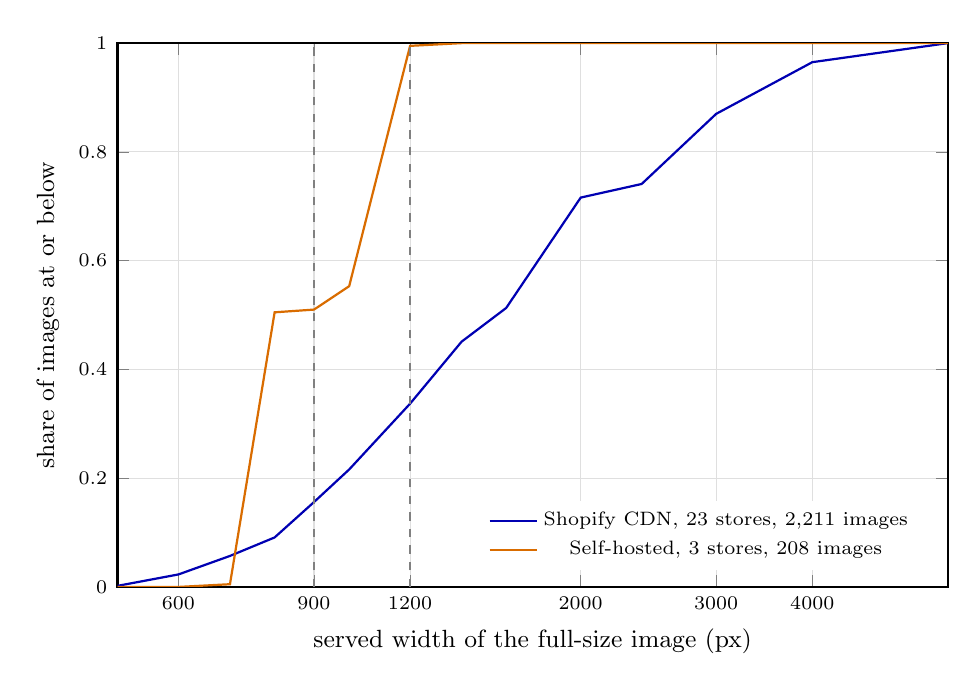
\begin{tikzpicture}
\begin{axis}[
  width=\columnwidth, height=0.7\columnwidth,
  xlabel={served width of the full-size image (px)}, ylabel={share of images at or below},
  xmode=log, log basis x=10, xmin=500, xmax=6000, ymin=0, ymax=1,
  xtick={600,900,1200,2000,3000,4000}, xticklabels={600,900,1200,2000,3000,4000},
  grid=major, grid style={gray!25},
  legend pos=south east, legend style={font=\scriptsize, draw=none},
  tick label style={font=\scriptsize}, label style={font=\small}, line width=0.8pt]
\addplot[color=blue!70!black, mark=none] coordinates {(500,0.002) (600,0.023) (700,0.057) (800,0.091) (900,0.156) (1000,0.216) (1200,0.337) (1400,0.451) (1600,0.513) (2000,0.716) (2400,0.741) (3000,0.870) (4000,0.965) (6000,1.000)};
\addlegendentry{Shopify CDN, 23 stores, 2,211 images}
\addplot[color=orange!85!black, mark=none] coordinates {(500,0.000) (600,0.000) (700,0.005) (800,0.505) (900,0.510) (1000,0.553) (1200,0.995) (1400,1.000) (6000,1.000)};
\addlegendentry{Self-hosted, 3 stores, 208 images}
\addplot[dashed, gray, no markers, forget plot] coordinates {(900,0) (900,1)};
\addplot[dashed, gray, no markers, forget plot] coordinates {(1200,0) (1200,1)};
\end{axis}
\end{tikzpicture}
\caption{Served width of full-size product images in 26 live stores, 15 October 2026. Dashed lines at 900 and 1,200\,px. The self-hosted step at 752\,px is one store's whole catalogue.}
\label{fig:widths}
\end{figure}

\section{Deployment constraints}
\label{sec:constraints}

The results above were obtained on one host with one editor. A pipeline that offers the same guarantees to other stores inherits four constraints that we analysed from the standards positions, platform discussions and libraries involved.

\subsection{Browser isolation}

Core sends Document-Isolation-Policy only on the post editor, site editor and widgets screens, only for Chromium 137 and later (Chrome on Android from 146), and only on devices with more than 2\,GB of memory, two cores, a connection faster than 2G and no Save-Data header; any failed check falls back to the server silently, and the worker download is about 13\,MB~\cite{wp71devnote}. Firefox and Safari always fall back. Mozilla's standards position moved to ``positive'' on 5 August 2026 without an implementation commitment~\cite{mozilla1074}; WebKit's only label is ``concerns: venue'' from 26 September 2026, asking for the mechanism to be upstreamed into Fetch and HTML~\cite{webkit399}; a proposal to include it in Interop 2027 is open~\cite{interop1332}. A plugin by the same WordPress contributor bridges the gap with the older headers (\texttt{credentialless} on Firefox, \texttt{require-corp} on Safari, which lacks \texttt{credentialless}) and documents the cost: embeds that need a session render logged out, third-party media without a CORP header fails, and OAuth popups hang~\cite{csme}. wasm-vips offers no single-threaded build; its maintainer states that libvips requires threads~\cite{wasmvips}.

The breakage, however, is a property of the editor page, which embeds third-party content, not of the headers. A dedicated bulk-processing administration page embeds nothing third-party and can send \texttt{COOP: same-origin} and \texttt{COEP: require-corp} in every browser today, provided its own scripts, fonts and images are same-origin or carry a CORP header. Browser-side bulk processing is therefore feasible across browsers now; browser-side processing inside the editor stays Chromium-only until Document-Isolation-Policy ships elsewhere.

\subsection{A perceptual metric in WebAssembly}

No WebAssembly build of SSIMULACRA~2 exists. The Rust implementation depends on \texttt{num-traits}, \texttt{thiserror}, \texttt{yuvxyb} and, optionally but by default, \texttt{rayon}~\cite{rustavssimulacra2}. Threads in Rust on the web require \texttt{SharedArrayBuffer}, a nightly toolchain and a rebuilt standard library~\cite{wasmbindgenrayon}; without threads, rayon on \texttt{wasm32} runs its two halves sequentially~\cite{rayoncore}. The metric itself needs no threads, so a build with default features off and one worker per image avoids the isolation requirement entirely. Single-threaded native implementations take 350 to 380\,ms at 1080p and 1.4 to 1.7\,s at 4K~\cite{zensim}; with the usual WebAssembly slowdown and three or four candidate encodings per image, a 2048\,px product photograph costs several seconds of one core, and a thousand-image library an hour or two of an administrator's laptop. The score must be validated against the reference command-line implementation before it is shown.

\subsection{Colour transform routes}

Measuring the loss is done; transforming pixels is not. GD cannot. ImageMagick converts through \texttt{profileImage} only when built with LittleCMS, and silently does nothing otherwise~\cite{phpimagick}; whether a shared host's build has the delegate is unknown until tested, and some phone files carry the P3 description only in EXIF rather than as an ICC profile, so the source profile must be assigned before conversion~\cite{imagemagickp3}. In the browser, libvips exposes \texttt{icc\_transform} with LittleCMS black-point compensation~\cite{libvipsicc}, but no documentation confirms that the WebAssembly build bundles LittleCMS; stand-alone WebAssembly and JavaScript ICC engines exist~\cite{lcmswasm,jscolorengine}. The browser's own decoder converts a tagged image when it is drawn onto an sRGB canvas, but the specification leaves that conversion implementation-defined and \texttt{createImageBitmap}'s \texttt{colorSpaceConversion: "default"} is explicitly implementation-specific~\cite{mdncreateimagebitmap}, and WebKit's canvas clips wide gamut to sRGB rather than mapping it~\cite{webkitwidegamut}; any browser route must be measured per browser with an image of known values. A pure-PHP matrix transform is correct but costs tens of seconds per 2048\,px image. The practical design is three tiers chosen per site by a capability check, with a second $\Delta E$ measurement after every transform as the proof.

\subsection{Platform evolution}

Browser-side processing covers uploads only; the 7.1 discussion mentions generating sizes on demand and adopting libvips on the server, neither committed~\cite{wp71devnote}. The WordPress Performance Team already distributes WebP and AVIF conversion, dominant-colour placeholders~\cite{dominantcolor} and, in beta, LCP prioritisation from field data~\cite{imageprioritizer}. Everything in the encoder and placeholder layer, including parts of this pipeline, should be expected to become platform functionality; the measurement, the colour guarantee and the quality target are the durable contributions.

\section{Threats to validity}

\textbf{External validity.} One store, one host, one editor for the pipeline and calibration. The 14\% prevalence of Display P3 is one library's number and reflects that its photographs came straight from a phone; the web-wide figure is 0.4\%~\cite{almanac2024media} and the live-store crawl found 0.5\%. That crawl is a hand-picked niche list, mostly Shopify, and measures served files only: a profile a host dropped before serving is invisible to it, and so is a shift that an export tool caused before upload. Its numbers are store properties sampled over 26 stores, three of them self-hosted, not image properties sampled over 2,419 images: the 13 wide-gamut images sit in two stores and the small images in three, so the sample supports the platform behaviours it observed and the size defect in this niche, not a prevalence estimate for self-hosted stores at large. A larger sample should come from a documented frame such as the HTTP Archive~\cite{httparchive}, drawn by platform and rank band and weighted towards self-hosted stores, where the colour question is open. The calibration uses six photographs per category, two for necklaces and one for bracelets. \textbf{Construct validity.} SSIM on luminance at half size is a proxy for perceived quality, not a perceptual metric; $\Delta E_{76}$ overstates differences in saturated regions relative to CIEDE2000~\cite{sharma2005ciede}; the colour sample is 48\,px wide. \textbf{Internal validity.} The Display P3 test profile was synthesised with the canonical primaries and parametric sRGB-type curves rather than taken from a device; timings on the web path include the local Apache configuration. \textbf{Conclusion validity.} The upload-path defect was reproduced twice with a cleaned library; its correction was tested on the real path and in isolation.

\section{Future work}

The crawl should move from a hand-picked list to a documented sampling frame such as the HTTP Archive, with enough self-hosted stores to estimate how many resize without colour management; the per-image thumbnail check already answers that question for every wide-gamut upload it finds. A pairwise viewing study on fabric colours would validate the 2.3 threshold and the three-tier transform. The SSIMULACRA~2 port, validated against the reference implementation, would replace the proxy score; an encode-until-pass loop on the browser-side path would then give every image its own quality.

\section{Conclusion}

The encoder layer of a storefront image pipeline is now platform functionality; what remains for a store to get right, and for tooling to prove, is quality and colour. On one real library, converting to WebP on the platform's own filters removed a third of the bytes without visible loss, a sequencing defect in the platform's new browser-side path was found and corrected, a per-category calibration showed that only a per-image perceptual target is both small and safe, and a profile measurement found that one photograph in seven carried a wide-gamut profile whose loss on the host's editor exceeds the visible threshold on every pixel. A crawl of 26 live catalogues then placed that finding: wide-gamut profiles are rare in served product images, the platforms sampled handle them correctly, and the colour risk is concentrated in self-hosted stores that resize without colour management and upload straight from a phone, while images too small for their box are the defect every kind of store shares. The constraints on doing the same for every store are concrete: document isolation limits browser-side processing to Chromium except on a dedicated page, a perceptual metric in WebAssembly is feasible but unported, and a colour transform on shared hosting must be chosen per site and verified by measurement.

\section*{Availability}

The colour measurement (the profile parser and the $\Delta E$ measure), the crawler for the multi-store study, the pixel check of the CDN copies, the calibration script, the synthetic Display P3 profile used for validation and the crawl data are published in the study repository~\cite{studyrepo}, as plain PHP with no dependency on WordPress or an imaging library. The crawler reads only public catalogues, honours \texttt{robots.txt}, fetches the header bytes of each full-size file and the thumbnail of each non-sRGB one, and reports prevalence separately for files that are the upload itself. The storefront pipeline of Section~\ref{sec:pipeline} and its tests are part of the merchant's theme and are not released; the three filters it answers and the correction of the finalize step are described in full in Sections~\ref{sec:pipeline} and~\ref{sec:paths}.

\bibliographystyle{ACM-Reference-Format}
\bibliography{refs}

\end{document}
